

\begin{frame}{Độ đo}
	\textbf{Mean opinion scores (MOS)}
%	Độ đo theo đánh giá của con người:
	
	\begin{itemize}
		\item Human-likeness
		\item Gesture-Speech Appropriateness
		\item Gesture-style Appropriateness
	\end{itemize}
	
	\textbf{FID (Fréchet Inception Distance)}: Sự tương đồng về phân phối của cử chỉ tạo sinh $\mathbf{g} \in \mathbb{R}^{1:M \times D}$ (generated) và $\mathbf{r} \in \mathbb{R}^{1:M \times D}$ (real)
%	\vspace{-5mm}
%	\begin{equation*}
%		\operatorname{FID} = \left\| \mu_{\operatorname{real}} - \mu_{\operatorname{predict}} \right\|^2 + \operatorname{Tr} \left( \Sigma_{\operatorname{real}} + \Sigma_{\operatorname{predict}} - 2 \left( \Sigma_{\operatorname{real}} \Sigma_{\operatorname{predict}} \right)^{\frac{1}{2}} \right)
%	\end{equation*}
	
	\begin{equation}
	FID = \left\| \mu_r - \mu_g \right\|^2 + \operatorname{Tr}\left( \Sigma_r + \Sigma_g - 2\sqrt{\Sigma_r \Sigma_g} \right)
	\end{equation}
	
%\begin{itemize}
%	\item $\mu_r$ và $\Sigma_r$ là vector trung bình và ma trận hiệp phương sai của đặc trưng từ dữ liệu thực tế (real gestures).
%	\item $\mu_g$ và $\Sigma_g$ là vector trung bình và ma trận hiệp phương sai của đặc trưng từ cử chỉ tổng hợp (generated gestures).
%	\item $\|\mu_r - \mu_g\|^2$ là bình phương khoảng cách Euclidean giữa các vector trung bình.
%	\item $\text{Tr}\left( \Sigma_r + \Sigma_g - 2\sqrt{\Sigma_r \Sigma_g} \right)$ là trace của ma trận hiệp phương sai kết hợp, đo lường sự khác biệt giữa hai phân phối Gaussian.
%\end{itemize}
	
	Trong đó
	\begin{itemize}
		\item $\mu$: Trung bình các đặc trưng của cử chỉ
		\item $\Sigma$: Ma trận hiệp phương sai, $\operatorname{Tr}$ là tổng đường chéo chính.
		\item $\sqrt{\Sigma_r \Sigma_g}$: Sự tương đồng giữa các phân phối.
	\end{itemize}
	
%	\begin{itemize}
%		\item \textbf{FID thấp}: Cho thấy phân phối của cử chỉ sinh ra rất gần với phân phối của cử chỉ thực tế, tức là cử chỉ tổng hợp trông tự nhiên hơn.
%		\item \textbf{FID cao}: Gợi ý rằng các cử chỉ sinh ra khác biệt nhiều so với các cử chỉ thực tế, tức là chất lượng kém hơn.
%	\end{itemize}
%	
\end{frame}
\begin{frame}{Kết quả}
	\begin{columns}
	\begin{column}{0.33\textwidth}
		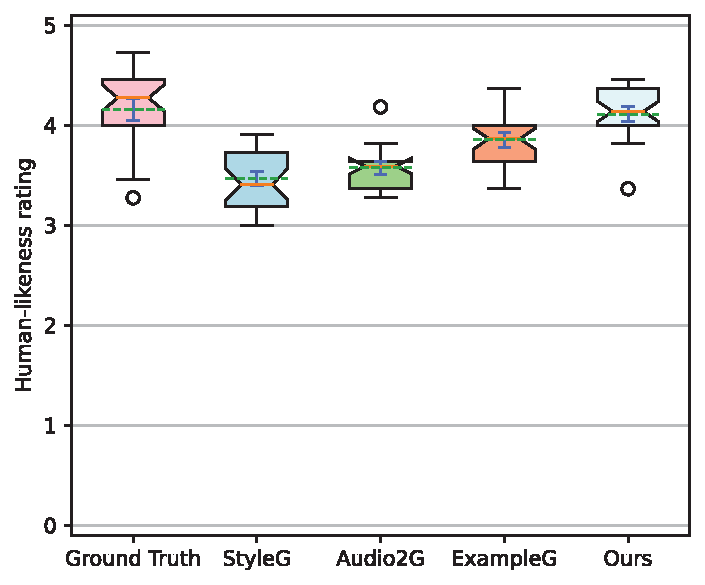
\includegraphics[width=\linewidth]{BoxHumanLikeness.pdf}
	\end{column}
	
	\begin{column}{0.33\textwidth}
		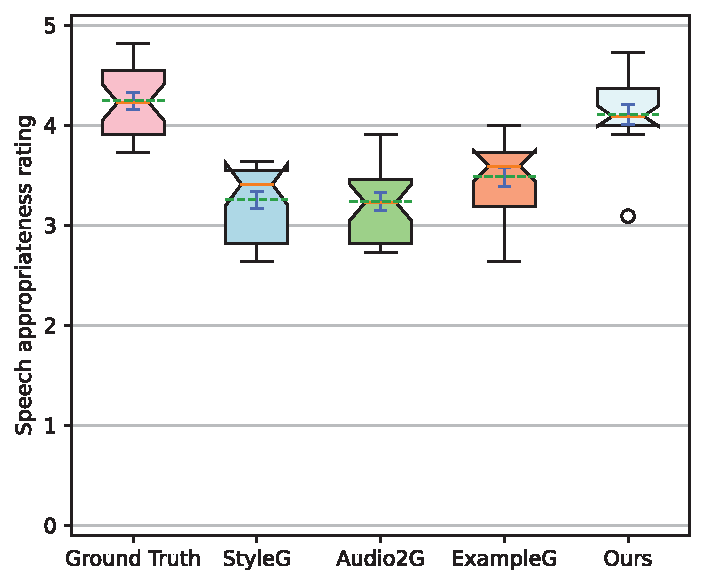
\includegraphics[width=\linewidth]{BoxSpeechAppropriateness.pdf}
	\end{column}
	
	\begin{column}{0.33\textwidth}
		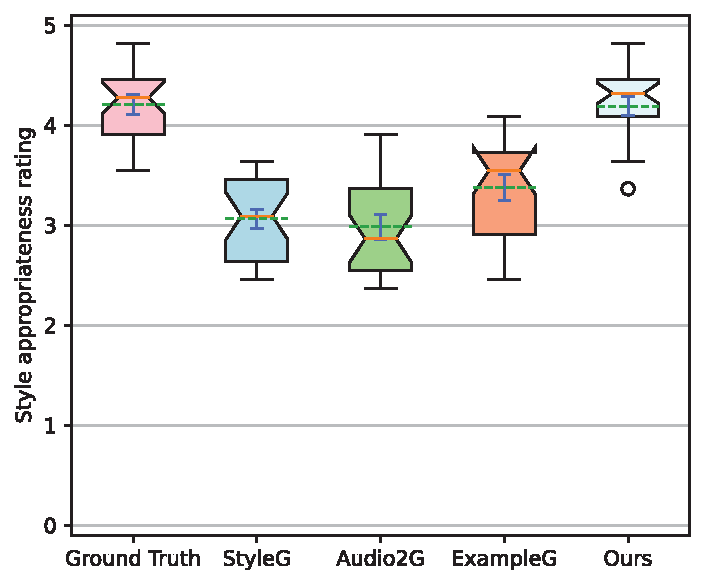
\includegraphics[width=\linewidth]{BoxStyleAppropriateness.pdf}
	\end{column}
\end{columns}

%Thử nghiệm với các thành phần cấu trúc trong mô hình:	
%
%\begin{enumerate}
%\item Sử dụng đặc trưng WavLM
%\item 
%\end{enumerate}

%\begin{itemize}
%	\item (1)sdf 
%\end{itemize}

\begin{table}[!t]
%	\footnotesize
\tiny
	\centering
	\resizebox{\columnwidth}{!}{%
		\begin{tabular}{lcc}
			\hline
			\multicolumn{1}{c}{Name} &
			\begin{tabular}[c]{@{}c@{}}Human\\ likeness \end{tabular}$\uparrow$ &
			\begin{tabular}[c]{@{}c@{}}Gesture-speech\\ appropriateness\end{tabular}$\uparrow$ \\ \hline
			Ground Truth          & 4.15 $\pm$ 0.11          & 4.25 $\pm$ 0.09          \\
			Ours                  & \textbf{4.11 $\pm$ 0.08} & \textbf{4.11 $\pm$ 0.10} \\
			\quad$-$ WavLM             & 4.05 $\pm$ 0.10          & 3.91 $\pm$ 0.11          \\
			\quad$-$ Cross-local attention   & 3.76 $\pm$ 0.09          & 3.51 $\pm$ 0.15          \\
			\quad$-$ Self-attention    & 3.55 $\pm$ 0.13          & 3.08 $\pm$ 0.10          \\
			% \begin{tabular}[c]{@{}c@{}}$-$ attention (GRU based) \\ (GRU based)\end{tabular} &
			\quad$-$ Attention + GRU&
			3.10 $\pm$ 0.11 &
			2.98 $\pm$ 0.14 \\
			\quad$+$ Forward attention & 3.75 $\pm$ 0.15          & 3.23 $\pm$ 0.24          \\
			\hline
		\end{tabular}%
	}
%	\caption{Kết quả của các nghiên cứu loại bỏ (Ablation studies). "$-$" chỉ các mô-đun không được sử dụng và "$+$" chỉ các mô-đun bổ sung. Chữ in đậm chỉ ra chỉ số tốt nhất.}
	\label{Ab}
\end{table}

\end{frame}
